\documentclass[tikz,border=3mm]{standalone}
\usepackage{pgfplots}
\pgfplotsset{compat=1.18}

\begin{document}
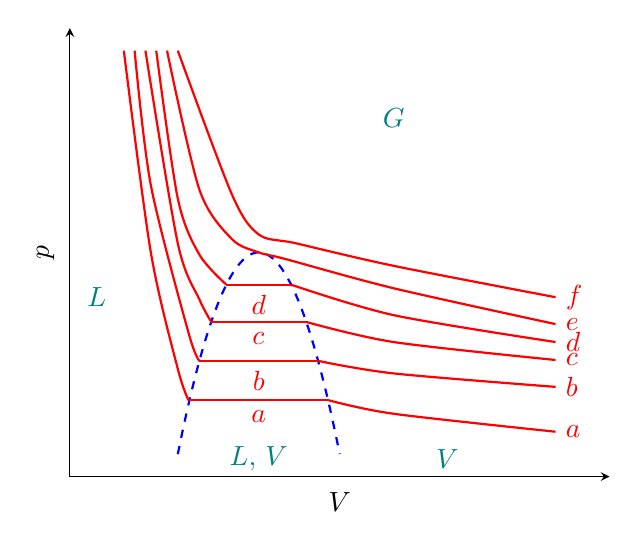
\begin{tikzpicture}
\begin{axis}[
    axis lines = left,
    xlabel = {$V$},
    ylabel = {$p$},
    xtick = \empty,
    ytick = \empty,
    xmin = 0, xmax = 10,
    ymin = 0, ymax = 10,
    domain = 1.5:8.5,
    samples = 100,
    legend pos = north east,
    legend style = {draw=none, fill=none}
]

    \addplot[blue, thick, dashed, domain=2:5] {-2*(\x-3.5)^2 +5 } ;

    \addplot[smooth, red, thick] coordinates {
        (1 , 9.5) (1.5, 5) (2,2.4) (2.2, 1.7)
    };
    \draw[red, thick] (2.2, 1.7)--(4.8, 1.7) node [midway, below] {$a$};
    \addplot[smooth, red, thick] coordinates {
        (4.8, 1.7) (6,1.4) (9, 1)
    } node [right] {$a$};

    
    \addplot[smooth, red, thick] coordinates {
        (1.2, 9.5) (1.5, 6.5) (2.2, 3.2) (2.4, 2.58)
    };
    \draw[red, thick] (2.4, 2.58)--(4.6, 2.58) node [midway, below] {$b$};
    \addplot[smooth, red, thick] coordinates {
        (4.6, 2.58) (6,2.3) (9, 2)
    } node [right] {$b$};

    \addplot[smooth, red, thick] coordinates {
        (1.4, 9.5) (2, 5.2) (2.4, 3.95) (2.62, 3.4512)
    };
    \draw[red, thick] (2.62, 3.4512)--(4.37, 3.4512) node [midway, below] {$c$};
    
    \addplot[smooth, red, thick] coordinates {
        (4.37, 3.4512) (6, 3) (9, 2.6)
    } node [right] {$c$};

    \addplot[smooth, red, thick] coordinates {
        (1.6, 9.5) (2, 6.2) (2.4, 4.95) (2.9, 4.28)
    };
    \draw[red, thick] (2.9, 4.28)--(4.1, 4.28) node [midway, below] {$d$};
    
    \addplot[smooth, red, thick] coordinates {
        (4.1, 4.28) (6, 3.6) (9, 3)
    } node [right] {$d$};

    \addplot[smooth, red, thick] coordinates {
        (1.8, 9.5) (2.4, 6.4) (3.0, 5.3) (3.5, 5)  (4, 4.85) (6, 4.2) (9, 3.4)
    } node [right] {$e$};

    \addplot[smooth, red, thick] coordinates {
        (2, 9.5)  (3.0, 6.3) (3.5, 5.4)  (4.2, 5.2) (6, 4.7) (9, 4)
    } node [right] {$f$};
    
    
    \node [teal] at (0.5, 4) {$L$};
    \node [teal] at (3.5, 0.4) {$L,\,V$};
    \node [teal] at (7, 0.4) {$V$};
    \node [teal] at (6, 8) {$G$};

\end{axis}
\end{tikzpicture}
\end{document}